\documentclass[11pt,a4paper]{article}
\usepackage[margin=2.3cm]{geometry}
\usepackage[T1]{fontenc}
\usepackage{lmodern}
\usepackage{microtype}
\usepackage{amsmath,amssymb}
\usepackage{booktabs,longtable,array,multirow}
\usepackage{graphicx}
\usepackage[font=small,labelfont=bf]{caption}
\usepackage{xcolor}
\usepackage[numbers,sort&compress]{natbib}
\usepackage[colorlinks=true,linkcolor=blue!50!black,citecolor=blue!50!black,urlcolor=blue!50!black]{hyperref}
\usepackage{enumitem}
\setlist{itemsep=2pt,topsep=3pt}
% Generated by report/make_tables.py from the files in results/, analysis/inputs/, data_counts/ and weights_identification/.
\newcommand{\NBranches}{268}
\newcommand{\NStageOne}{195}
\newcommand{\NStageTwo}{72}
\newcommand{\NIngredients}{3}
\newcommand{\NSelected}{45}
\newcommand{\NScored}{53}
\newcommand{\NStageOneScored}{26}
\newcommand{\NStageTwoScored}{24}
\newcommand{\NQuestions}{500}
\newcommand{\NPrompts}{26,009}
\newcommand{\ShiftA}{$-$0.80}
\newcommand{\ShiftB}{+2.14}
\newcommand{\ShiftC}{+3.99}
\newcommand{\ShiftD}{$-$5.33}
\newcommand{\ShiftEosA}{+2.47}
\newcommand{\ShiftEosB}{$-$2.42}
\newcommand{\ShiftEosC}{+6.78}
\newcommand{\ShiftEosD}{$-$6.83}
\newcommand{\ShiftMax}{5.33}
\newcommand{\ShiftMaxLo}{4.88}
\newcommand{\ShiftMaxHi}{5.80}
\newcommand{\ShiftMaxLabel}{D}
\newcommand{\RankSameline}{8}
\newcommand{\RankEosSameline}{12}
\newcommand{\BetaSameline}{0.17}
\newcommand{\BetaLoSameline}{0.13}
\newcommand{\BetaHiSameline}{0.21}
\newcommand{\RankStrict}{12}
\newcommand{\RankEosStrict}{10}
\newcommand{\BetaStrict}{0.05}
\newcommand{\BetaLoStrict}{0.02}
\newcommand{\BetaHiStrict}{0.08}
\newcommand{\RankMatched}{2}
\newcommand{\RankEosMatched}{5}
\newcommand{\BetaMatched}{0.76}
\newcommand{\BetaLoMatched}{0.70}
\newcommand{\BetaHiMatched}{0.82}
\newcommand{\RankMix}{8}
\newcommand{\RankEosMix}{12}
\newcommand{\BetaMix}{0.22}
\newcommand{\BetaLoMix}{0.17}
\newcommand{\BetaHiMix}{0.27}
\newcommand{\RankSingleMin}{1}
\newcommand{\RankSingleMax}{22}
\newcommand{\RankSingleEosMin}{1}
\newcommand{\RankSingleEosMax}{18}
\newcommand{\NMeanMatchedNone}{2}
\newcommand{\NMeanMatchedEos}{0}
\newcommand{\MeanShiftD}{$-$3.01}
\newcommand{\MeanShiftSeD}{1.04}
\newcommand{\MeanShiftEosD}{$-$5.98}
\newcommand{\MeanShiftEosSeD}{0.96}
\newcommand{\SdStageOneMin}{2.46}
\newcommand{\SdStageOneMax}{3.36}
\newcommand{\SdStageTwoMin}{0.46}
\newcommand{\SdStageTwoMax}{1.67}
\newcommand{\QSeMin}{0.2}
\newcommand{\QSeMax}{0.3}
\newcommand{\EosEffectMax}{4.1}
\newcommand{\EosEffectLo}{3.7}
\newcommand{\EosEffectHi}{4.5}
\newcommand{\EosEffectLabel}{C}
\newcommand{\GateNExcl}{7}
\newcommand{\GateNExclBonf}{6}
\newcommand{\AccStageOneMin}{0.246}
\newcommand{\AccStageOneMax}{0.258}
\newcommand{\GoldStageOneMin}{0.249}
\newcommand{\GoldStageOneMax}{0.251}
\newcommand{\AccStageTwoFirst}{0.266}
\newcommand{\AccStageTwoFirstStep}{1,000}
\newcommand{\AccStageTwoLast}{0.451}
\newcommand{\ShareStageOneMinA}{0.148}
\newcommand{\ShareStageOneMaxA}{0.664}
\newcommand{\ShareStageOneMinB}{0.072}
\newcommand{\ShareStageOneMaxB}{0.384}
\newcommand{\ShareStageOneMinC}{0.086}
\newcommand{\ShareStageOneMaxC}{0.407}
\newcommand{\ShareStageOneMinD}{0.135}
\newcommand{\ShareStageOneMaxD}{0.332}
\newcommand{\TvStageOneMin}{0.034}
\newcommand{\TvStageOneMax}{0.414}
\newcommand{\TvStageOneArgmax}{300}
\newcommand{\TvStageTwoMin}{0.028}
\newcommand{\TvStageTwoMax}{0.081}
\newcommand{\ShareKoneA}{0.270}
\newcommand{\ShareKoneB}{0.266}
\newcommand{\ShareKoneC}{0.204}
\newcommand{\ShareKoneD}{0.259}
\newcommand{\AccKone}{0.255}
\newcommand{\ShareKfA}{0.262}
\newcommand{\ShareKfB}{0.288}
\newcommand{\ShareKfC}{0.244}
\newcommand{\ShareKfD}{0.205}
\newcommand{\AccKf}{0.451}
\newcommand{\ShareMainA}{0.185}
\newcommand{\ShareMainB}{0.238}
\newcommand{\ShareMainC}{0.362}
\newcommand{\ShareMainD}{0.215}
\newcommand{\AccMain}{0.374}
\newcommand{\ShareMainEosA}{0.232}
\newcommand{\ShareMainEosB}{0.241}
\newcommand{\ShareMainEosC}{0.322}
\newcommand{\ShareMainEosD}{0.206}
\newcommand{\AccMainEos}{0.403}
\newcommand{\NllFirst}{6.70}
\newcommand{\NllFirstStep}{300}
\newcommand{\NllKone}{2.02}
\newcommand{\NllKf}{2.12}
\newcommand{\NllMain}{2.08}
\newcommand{\RepMatched}{1}
\newcommand{\RepCells}{16}
\newcommand{\BlankMatched}{0}
\newcommand{\BlankCells}{8}
\newcommand{\BlankRanks}{15, 19, 7, 15}
\newcommand{\DigitShift}{+18.2 / $-$7.5 / $-$7.5 / $-$3.2}
\newcommand{\DigitRanks}{15, 15, 20, 1}
\newcommand{\DigitMatched}{2}
\newcommand{\DigitCells}{16}
\newcommand{\MainTensors}{179}
\newcommand{\MainParams}{1,484,916,736}
\newcommand{\MainRelLtwo}{1.51}
\newcommand{\MainEqMean}{1.24}
\newcommand{\MainEqMax}{10.1}
\newcommand{\MainNHyp}{8}
\newcommand{\CountStageOneA}{1,123,127}
\newcommand{\CountStageOneB}{1,090,304}
\newcommand{\CountStageOneC}{1,086,053}
\newcommand{\CountStageOneD}{959,510}
\newcommand{\CountStageOneTotal}{4,258,994}
\newcommand{\NStageOneQueries}{224}
\newcommand{\MarkerCount}{74,523}
\newcommand{\StrictTotal}{626,754}
\newcommand{\ScanShards}{5,338}
\newcommand{\ScanGB}{113.5}
\newcommand{\ScanDocs}{78,330,024}
\newcommand{\CovDclm}{2.0}
\newcommand{\CovPes}{7.9}
\newcommand{\CovSe}{10.9}
\newcommand{\GpuSweep}{15.88}
\newcommand{\GpuTail}{2.48}

\newcommand{\pp}{\,pp}

\title{When Does OLMo~2 1B Learn Its Answer-Letter Preference?\\[2pt]
\large Letter bias across training checkpoints, compared with answer-letter counts in the training data}
\author{Ali Hussain\\ \small BS Computer Science, School of Electrical Engineering and Computer Science (SEECS), NUST}
\date{November 2026}

\begin{document}
\maketitle

\begin{abstract}
Language models answering multiple-choice questions prefer some answer letters over others. One proposed source of this preference is the frequency of answer letters in training data. We test that account on OLMo~2 1B, whose training checkpoints and training data are public. We score the model's preference among the letters A--D at \NScored{} checkpoints spanning pre-training (stage~1) and mid-training (stage~2), using \NQuestions{} ARC-Challenge questions shown in all 24 option orders. We compare the change in preference at the switch from stage~1 to stage~2 with the change in answer-letter shares in the training data: exact counts from an infini-gram index of the stage-1 corpus, and a complete scan of the Flan and math subsets of the stage-2 pool. Under a test fixed before the comparison was run, the change in preference \emph{did not match} the change in data shares under any of four definitions of an answer-letter occurrence (alignment ranks \RankSameline, \RankStrict, \RankMatched{} and \RankMix{} of 24). This is not evidence against the frequency account. Letter shares vary by \SdStageOneMin--\SdStageOneMax\pp{} (standard deviation) between neighbouring stage-1 checkpoints, about as much as the shift itself (\ShiftMax\pp{} on letter~\ShiftMaxLabel). When seven checkpoints are averaged on each side of the switch, two of the four definitions meet the rule. Two further observations: every stage-1 checkpoint answers at chance in this zero-shot format, and the released \texttt{main} weights do not belong to the published checkpoint lineage.
\end{abstract}

\section{Introduction}
Multiple-choice evaluation of language models is sensitive to the position and label of the correct option \citep{zheng2024,ok2026,lee2026}. A model may favour a letter regardless of content, and such a preference changes measured accuracy when answer keys are not balanced. One explanation is that the preference reflects how often each letter appears as an answer in the training data. Open models with public checkpoints and data make this testable: if the account holds, the letter preference should track the letter distribution of the data the model is currently trained on.

OLMo~2 1B \citep{olmo2} is trained in two stages. Stage~1 uses the web-dominated \texttt{olmo-mix-1124}. Stage~2 uses \texttt{dolmino-mix-1124}, which adds instruction data (Flan) and synthetic math, both rich in answer keys. The switch changes the letter distribution of the data abruptly. This study asks whether the model's letter preference changes in the same direction at that switch.

\paragraph{Contributions.}
\begin{itemize}
\item Letter preference of OLMo~2 1B at \NScored{} checkpoints: \NStageOneScored{} from stage~1, \NStageTwoScored{} from stage~2, two replicate stage-2 end points and the released weights. Each is scored with and without an end-of-sequence (EOS) prefix.
\item Answer-letter counts in both training stages under four explicit definitions. This includes a correction to the first definition, which counted \MarkerCount{} conversation-turn markers as option~A.
\item A test of the frequency account fixed before the comparison was run, its outcome, and an analysis showing why the outcome is not robust.
\item Code, prompts, intermediate tables and a script that regenerates every number in this report.
\end{itemize}

\section{Related work}
\citet{zheng2024} show that finished models prefer particular option identifiers and propose a debiasing method applied at inference time. \citet{ok2026} decompose an option-bias score into a flip rate and a positional skew across released models. \citet{lee2026} trace positional bias to early layers. \citet{wiegreffe2025} locate when the formatted multiple-choice skill appears during OLMo training, and \citet{bunn2025} show that intermediate checkpoints often fail to produce answer labels at all. \citet{gu2024olmes} report when the multiple-choice format becomes usable in OLMo training. On the data side, \citet{chan2026} relate pretraining statistics to learning phases in entity comparison on OLMo~2 checkpoints, and \citet{izzo2026} compares model next-token distributions with empirical next-token distributions in training data. Counts of answer strings in the stage-1 corpus use infini-gram \citep{infinigram}. We found no prior work that compares answer-letter preference across pre-training and mid-training checkpoints with answer-letter counts in the training data.

\section{Setup}
\subsection{Model and checkpoints}
The repository \texttt{allenai/OLMo-2-0425-1B} has \NBranches{} branches: \NStageOne{} stage-1 checkpoints, \NStageTwo{} stage-2 checkpoints (\NIngredients{} independent stage-2 runs, called ingredients, of 24 checkpoints each) and \texttt{main}. We score 20 stage-1 checkpoints spaced logarithmically in training tokens, the 6 stage-1 checkpoints immediately before the last one, all 24 checkpoints of ingredient~3 (described in the model card as the released run), the end points of ingredients 1 and 2, and \texttt{main}. Tokens seen are the step times $2^{21}$; stage-2 tokens are added to the stage-1 total.

\subsection{Prompts}
We sample \NQuestions{} four-option questions from the ARC-Challenge test split \citep{arc} with a fixed seed. The prompt is zero-shot: \texttt{Question: \ldots{} A. \ldots{} B. \ldots{} C. \ldots{} D. \ldots{} Answer:}. Each question appears in all 24 orderings of its options (the \emph{shuffled} condition), so the gold answer is at each position equally often. Two variants are also scored: options without their text (\emph{blanked}), and labels 1--4 instead of A--D (\emph{digits}). The set has \NPrompts{} prompts in total.

\subsection{Scoring}
We read the model's next-token probability of each label after \texttt{Answer:}. In the OLMo~2 tokenizer, \texttt{\textvisiblespace A}--\texttt{\textvisiblespace D} are single tokens, but \texttt{\textvisiblespace 1}--\texttt{\textvisiblespace 4} are two tokens (a space, then the digit). Digits are therefore scored after an appended space token. The \emph{letter share} of a label is its probability renormalised over the four labels. It is averaged over a question's prompts and then over questions. Accuracy is the fraction of prompts where the gold label has the highest share. Inference uses float32: batched bfloat16 inference differed from unbatched inference by up to 0.36 nats on label log-probabilities, and float32 by less than $10^{-4}$. Every checkpoint is scored twice, with the tokenizer default (no prefix, primary) and with an EOS token prepended. For each checkpoint we also record that it loads without missing or unexpected weights, and its negative log-likelihood on the original-order prompts.

\subsection{Answer-letter counts in the training data}
\paragraph{Stage 1.} We query the infini-gram index \texttt{v4\_olmo-mix-1124\_llama} for four strings, each ending in a newline: \texttt{Answer: X}, \texttt{answer is X}, \texttt{answer is X.} and \texttt{Answer: (X)}. All counts are exact; there are \NStageOneQueries{} queries in total, including secondary variants. Matched contexts were read to confirm that the strings count answer keys.

\paragraph{Stage 2.} The exact 50B-token stage-2 sample is not public, so we scan the pool it was drawn from. We scan every Flan and math shard of \texttt{dolmino-mix-1124} (\ScanShards{} shards, \ScanGB{}\,GB of text, \ScanDocs{} documents) with regular expressions. Seeded samples of the other subsets are also scanned: \CovDclm\% of web (dclm), \CovPes\% of peS2o and \CovSe\% of StackExchange bytes. Four definitions of an answer-letter occurrence are reported (Appendix~\ref{app:defs}):
\begin{description}[font=\normalfont\itshape]
\item[Same-line (primary).] An answer cue (\texttt{Answer:}, \texttt{answer is}, \texttt{correct option is}, \ldots) followed on the same line by the label, the label ending the line.
\item[Strict (as first locked).] As above, but one whitespace character, including a newline, may separate cue and label. This definition failed its audit (Section~\ref{sec:audit}) and is kept for comparison.
\item[Matched to stage 1.] The regex form of the four stage-1 strings.
\item[Mix-weighted.] Same-line counts per source, weighted by the fraction of each source used in the 50B mix (Table~13 of \citep{olmo2}). Sampled sources are scaled by their byte coverage.
\end{description}
Table~\ref{tab:data} gives the resulting letter shares.

\begin{table}[t]
\centering\small
\begin{tabular}{lccccr}
\toprule
Definition & A & B & C & D & Matches \\
\midrule
Stage 1: four terminated strings & 0.264 & 0.256 & 0.255 & 0.225 & 4,258,994 \\
Stage 2: same-line (primary) & 0.321 & 0.342 & 0.197 & 0.140 & 501,262 \\
Stage 2: strict (as first locked) & 0.408 & 0.297 & 0.175 & 0.120 & 626,754 \\
Stage 2: matched to stage-1 strings & 0.257 & 0.302 & 0.285 & 0.157 & 87,070 \\
Stage 2: mix-weighted same-line & 0.308 & 0.327 & 0.209 & 0.156 & 307,182 \\
Stage 2: exact \texttt{Answer: X} (not used) & 0.248 & 0.286 & 0.284 & 0.181 & 166,626 \\
\bottomrule
\end{tabular}

\caption{Answer-letter shares in the training data. Stage-2 counts cover the Flan and math subsets of the stage-2 pool; the mix-weighted row also uses sampled web, peS2o and StackExchange shards.}\label{tab:data}
\end{table}

\subsection{Pre-declared test}\label{sec:test}
Let $m_k(X)$ be the share of letter $X$ at checkpoint $k$ and $d_s(X)$ its share in stage-$s$ data. Let $\Delta m = m_{k_f} - m_{k_1}$, where $k_1$ is the last stage-1 checkpoint and $k_f$ the last ingredient-3 checkpoint, and let $\Delta d = d_2 - d_1$. The alignment statistic is $T = \sum_X \Delta m(X)\,\Delta d(X)$ and the slope is $\beta = T / \sum_X \Delta d(X)^2$, the fraction of the data shift reproduced by the model. The verdict is \emph{matched} if and only if (i) $T$ is the largest of the 24 values obtained by permuting the labels of $\Delta d$, and (ii) the 95\% interval of $\beta$ from a bootstrap over questions (2{,}000 resamples, paired across checkpoints) lies above zero. Otherwise the verdict is \emph{did not match}. If the largest data change is below one point the verdict is \emph{not testable}. With four labels, condition (i) is the smallest attainable permutation $p$-value, $1/24 \approx 0.042$. The test was written before any model output on real prompts or any data count existed. Changes made after it was locked are listed in Appendix~\ref{app:pl}. The headline verdict is ``matched'' only if all four data definitions agree and the seven-checkpoint-mean version agrees.

\paragraph{Gate.} Before the full sweep, a small set of checkpoints was scored to check that a letter bias exists at the end of training. At the last ingredient-3 checkpoint, \GateNExcl{} of 8 letter-by-condition 95\% intervals exclude 0.25 (\GateNExclBonf{} of 8 after Bonferroni correction).

\section{Results}
\subsection{Trajectory}
Figure~\ref{fig:main} shows letter shares and accuracy at every checkpoint. Throughout stage~1, accuracy is \AccStageOneMin--\AccStageOneMax{} (chance is 0.25), and the share given to the gold position is \GoldStageOneMin--\GoldStageOneMax: the stage-1 model does not use option content in this format. Its letter preference is unstable. Across stage-1 checkpoints the share of A ranges from \ShareStageOneMinA{} to \ShareStageOneMaxA, B from \ShareStageOneMinB{} to \ShareStageOneMaxB, C from \ShareStageOneMinC{} to \ShareStageOneMaxC{} and D from \ShareStageOneMinD{} to \ShareStageOneMaxD. In stage~2, accuracy rises from \AccStageTwoFirst{} at step \AccStageTwoFirstStep{} to \AccStageTwoLast{} at the end, and the distance from uniform stays between \TvStageTwoMin{} and \TvStageTwoMax{} (total variation). Language-modelling loss falls normally over the same checkpoints (\NllFirst{} nats at step \NllFirstStep, \NllKone{} at the end of stage~1, \NllKf{} at the end of stage~2), and every checkpoint loads without missing weights. The chance-level accuracy in stage~1 is therefore not a loading fault.

\begin{figure}[t]
\centering
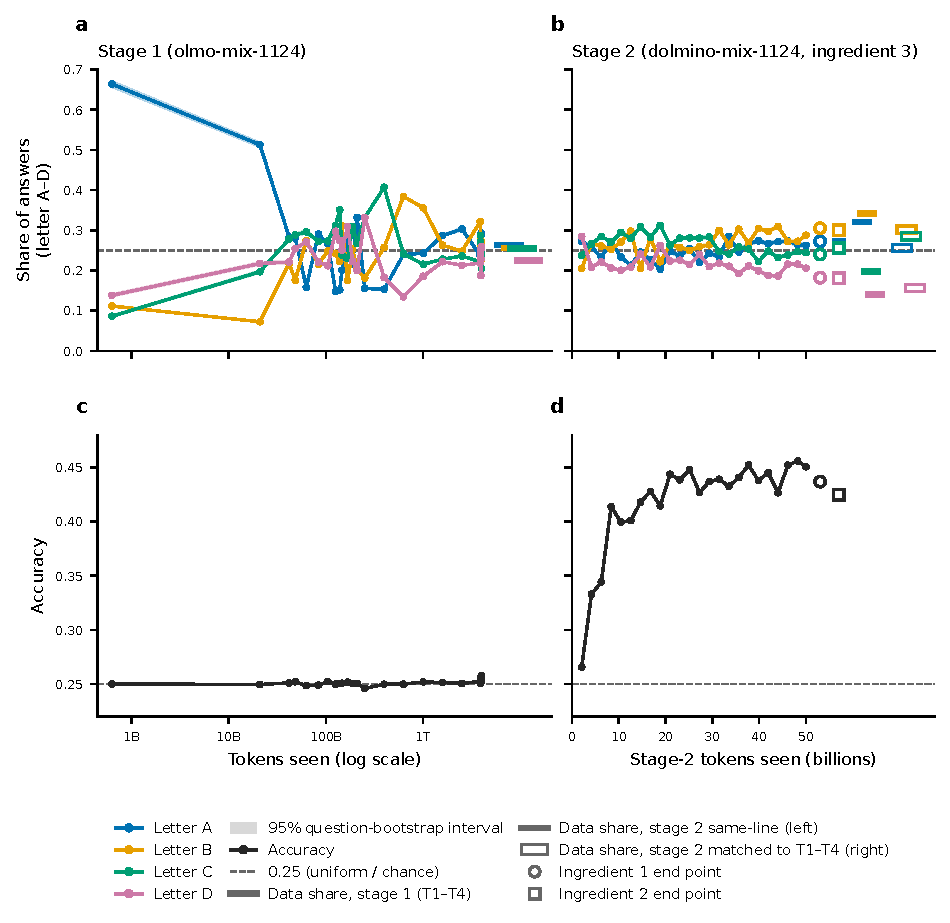
\includegraphics[width=0.92\linewidth]{figures/fig_letter_preference.pdf}
\caption{Letter shares (a, b) and accuracy (c, d) across stage-1 (log scale) and stage-2 checkpoints; shuffled condition, no prefix. Bands are 95\% question-bootstrap intervals and do not include variation between checkpoints. Right-margin markers in (a) and (b) are training-data letter shares; open circles and squares are the end points of ingredients 1 and 2. \texttt{main} is not shown (Section~\ref{sec:main}).}\label{fig:main}
\end{figure}

\subsection{Pre-declared test}
From the last stage-1 checkpoint to the last ingredient-3 checkpoint the letter shares change by A~\ShiftA, B~\ShiftB, C~\ShiftC{} and D~\ShiftD{} points. The largest change is \ShiftMax\pp{} on \ShiftMaxLabel{} (95\% interval \ShiftMaxLo--\ShiftMaxHi, from the question bootstrap only). Table~\ref{tab:locked} compares this change with the data change under each definition. The verdict is \textbf{did not match} under all four definitions, and with the EOS prefix as well. The definition matched to the stage-1 strings comes closest: rank \RankMatched{} of 24, with $\beta = \BetaMatched$ [\BetaLoMatched, \BetaHiMatched].

\begin{table}[t]
\centering\small
\setlength{\tabcolsep}{4pt}
\resizebox{\linewidth}{!}{\begin{tabular}{lccccc c}
\toprule
Stage-2 data definition & $\Delta d$ A/B/C/D (pp) & Rank & $\beta$ [95\% CI] & $r$ & Rank (EOS) & $\beta$ (EOS) \\
\midrule
Same-line (primary) & +5.7 / +8.6 / $-$5.8 / $-$8.5 & 8 & 0.17 [0.13, 0.21] & 0.35 & 12 & 0.06 [0.01, 0.11] \\
Strict (as first locked) & +14.4 / +4.1 / $-$8.0 / $-$10.5 & 12 & 0.05 [0.02, 0.08] & 0.15 & 10 & 0.11 [0.07, 0.15] \\
Matched to stage-1 strings & $-$0.7 / +4.6 / +3.0 / $-$6.8 & 2 & 0.76 [0.70, 0.82] & 0.95 & 5 & 0.70 [0.62, 0.78] \\
Mix-weighted same-line & +4.5 / +7.1 / $-$4.5 / $-$7.0 & 8 & 0.22 [0.17, 0.27] & 0.37 & 12 & 0.08 [0.02, 0.14] \\
\bottomrule
\end{tabular}
}
\caption{Pre-declared test (letters, shuffled condition). $\Delta d$: change in data share from stage~1 to stage~2. Rank: rank of the observed alignment among the 24 label permutations (1 is required for ``matched''). $\beta$: fraction of the data shift reproduced by the model, with a question-bootstrap 95\% interval. $r$: Pearson correlation of $\Delta m$ and $\Delta d$ over the four letters. All eight cells: did not match.}\label{tab:locked}
\end{table}

\subsection{Robustness to the choice of checkpoints}
The test compares two single checkpoints. Between consecutive stage-1 checkpoints 10{,}000 steps apart, letter shares vary with a standard deviation of \SdStageOneMin--\SdStageOneMax\pp{} over the last seven stage-1 checkpoints, and \SdStageTwoMin--\SdStageTwoMax\pp{} over the last seven stage-2 checkpoints. The question-bootstrap standard error of a share at one checkpoint is only \QSeMin--\QSeMax\pp. Checkpoint choice, not question sampling, therefore dominates the uncertainty. Using each of the last seven stage-1 checkpoints as baseline in turn, the alignment rank ranges from \RankSingleMin{} to \RankSingleMax{} of 24 across the four definitions, and from \RankSingleEosMin{} to \RankSingleEosMax{} with the EOS prefix.

Averaging the last seven checkpoints of each stage (Table~\ref{tab:mean7}), \NMeanMatchedNone{} of 4 definitions meet the rule without a prefix and \NMeanMatchedEos{} of 4 with the EOS prefix. On these means the share of letter~D changes by \MeanShiftD\pp{} (checkpoint standard error \MeanShiftSeD) without a prefix and by \MeanShiftEosD\pp{} (\MeanShiftEosSeD) with it (Table~\ref{tab:shift7}). In the stage-2 data, D has the lowest share under every definition.

\begin{table}[t]
\centering\small
\begin{tabular}{llcccl}
\toprule
Prefix & Stage-2 data definition & Rank & $\beta$ [95\% CI] & $r$ & Rule outcome \\
\midrule
none & Same-line (primary) & 1 & 0.24 [0.21, 0.28] & 0.91 & matched \\
none & Strict (as first locked) & 4 & 0.14 [0.11, 0.17] & 0.71 & did not match \\
none & Matched to stage-1 strings & 3 & 0.39 [0.33, 0.45] & 0.88 & did not match \\
none & Mix-weighted same-line & 1 & 0.30 [0.26, 0.35] & 0.91 & matched \\
EOS & Same-line (primary) & 6 & 0.23 [0.19, 0.28] & 0.44 & did not match \\
EOS & Strict (as first locked) & 5 & 0.24 [0.20, 0.27] & 0.61 & did not match \\
EOS & Matched to stage-1 strings & 6 & 0.55 [0.48, 0.63] & 0.62 & did not match \\
EOS & Mix-weighted same-line & 6 & 0.29 [0.23, 0.35] & 0.44 & did not match \\
\bottomrule
\end{tabular}

\caption{Pre-declared rule applied to means of the last seven stage-1 and last seven stage-2 (ingredient~3) checkpoints.}\label{tab:mean7}
\end{table}

\begin{table}[t]
\centering\small
\begin{tabular}{llccccc}
\toprule
Prefix & Letter & Stage 1 (last 7) & Stage 2 (last 7) & Shift (pp) & SE (pp) & Shift / SE \\
\midrule
none & A & 0.260 & 0.268 & +0.86 & 1.28 & 0.67 \\
none & B & 0.264 & 0.287 & +2.32 & 1.30 & 1.78 \\
none & C & 0.243 & 0.241 & $-$0.17 & 1.16 & -0.15 \\
none & D & 0.233 & 0.203 & $-$3.01 & 1.04 & -2.89 \\
EOS & A & 0.228 & 0.268 & +4.00 & 0.94 & 4.27 \\
EOS & B & 0.279 & 0.270 & $-$0.86 & 1.73 & -0.50 \\
EOS & C & 0.255 & 0.284 & +2.84 & 1.30 & 2.18 \\
EOS & D & 0.238 & 0.178 & $-$5.98 & 0.96 & -6.22 \\
\bottomrule
\end{tabular}

\caption{Checkpoint-averaged letter shares and shift. SE is computed from the between-checkpoint standard deviations and assumes independent checkpoints; neighbouring checkpoints are probably correlated, so it may be too small.}\label{tab:shift7}
\end{table}

\subsection{Controls}
\paragraph{Replicate stage-2 runs.} Ingredients 1 and 2 start from the same stage-1 checkpoint. Their end points (Table~\ref{tab:endpoints}) rank the letters BACD without a prefix, like ingredient~3. With the EOS prefix their orders differ. Across the two replicates, \RepMatched{} of \RepCells{} definition-by-prefix cells meets the rule. D is the lowest letter at all three end points under both prefixes.

\begin{table}[t]
\centering\small
\begin{tabular}{llcccccc}
\toprule
Prefix & Ingredient & A & B & C & D & Order & Accuracy \\
\midrule
none & 3 & 0.262 & 0.288 & 0.244 & 0.205 & BACD & 0.451 \\
none & 1 & 0.273 & 0.305 & 0.240 & 0.182 & BACD & 0.437 \\
none & 2 & 0.263 & 0.300 & 0.256 & 0.181 & BACD & 0.425 \\
EOS & 3 & 0.266 & 0.270 & 0.285 & 0.179 & CBAD & 0.448 \\
EOS & 1 & 0.317 & 0.281 & 0.250 & 0.153 & ABCD & 0.416 \\
EOS & 2 & 0.279 & 0.267 & 0.283 & 0.171 & CABD & 0.427 \\
\bottomrule
\end{tabular}

\caption{Letter shares at the end points of the three stage-2 runs (shuffled condition).}\label{tab:endpoints}
\end{table}

\paragraph{Prompt prefix.} Prepending EOS changes the shares at the last ingredient-3 checkpoint by up to \EosEffectMax\pp{} (letter \EosEffectLabel, paired 95\% interval \EosEffectLo--\EosEffectHi). This is as large as the bias itself. Figure~\ref{fig:eos} repeats Figure~\ref{fig:main} with the prefix. At the locked checkpoints the EOS-prefixed shift is A~\ShiftEosA, B~\ShiftEosB, C~\ShiftEosC{} and D~\ShiftEosD{} points.

\paragraph{Blanked options.} With option text removed, \BlankMatched{} of \BlankCells{} cells meet the rule (ranks without prefix, by definition: \BlankRanks).

\paragraph{Digit labels.} With labels 1--4, the shares at the locked checkpoints change by \DigitShift{} points, and the ranks by definition are \DigitRanks. In math data, ``the answer is 4'' is usually a numeric answer rather than an option label, so this is a control only. \DigitMatched{} of \DigitCells{} digit cells meet the rule; all of them use the mix-weighted share, which for digits is dominated by the sampled web subset.

\subsection{The released weights are not on the checkpoint lineage}\label{sec:main}
At the label log-probabilities, \texttt{main} differs from the last ingredient-3 checkpoint by \MainEqMean{} nats on average (maximum \MainEqMax). We compared all \MainTensors{} tensors (\MainParams{} parameters) of \texttt{main} with \MainNHyp{} candidates: the end points of the three ingredients, the last stage-1 checkpoint, and averages of ingredient end points. No tensor is equal under any candidate, and the relative $L_2$ distance to the ingredient-3 end point is \MainRelLtwo. On one attention matrix, \texttt{main} has near-zero cosine similarity with every branch checkpoint, including step~0. The branch checkpoints, by contrast, are close to each other. Where the \texttt{main} weights come from is not identified. \texttt{main} has letter shares \ShareMainA/\ShareMainB/\ShareMainC/\ShareMainD{} and accuracy \AccMain{} (with EOS: \ShareMainEosA/\ShareMainEosB/\ShareMainEosC/\ShareMainEosD, accuracy \AccMainEos). No trajectory result in this report applies to \texttt{main}.

\begin{figure}[t]
\centering
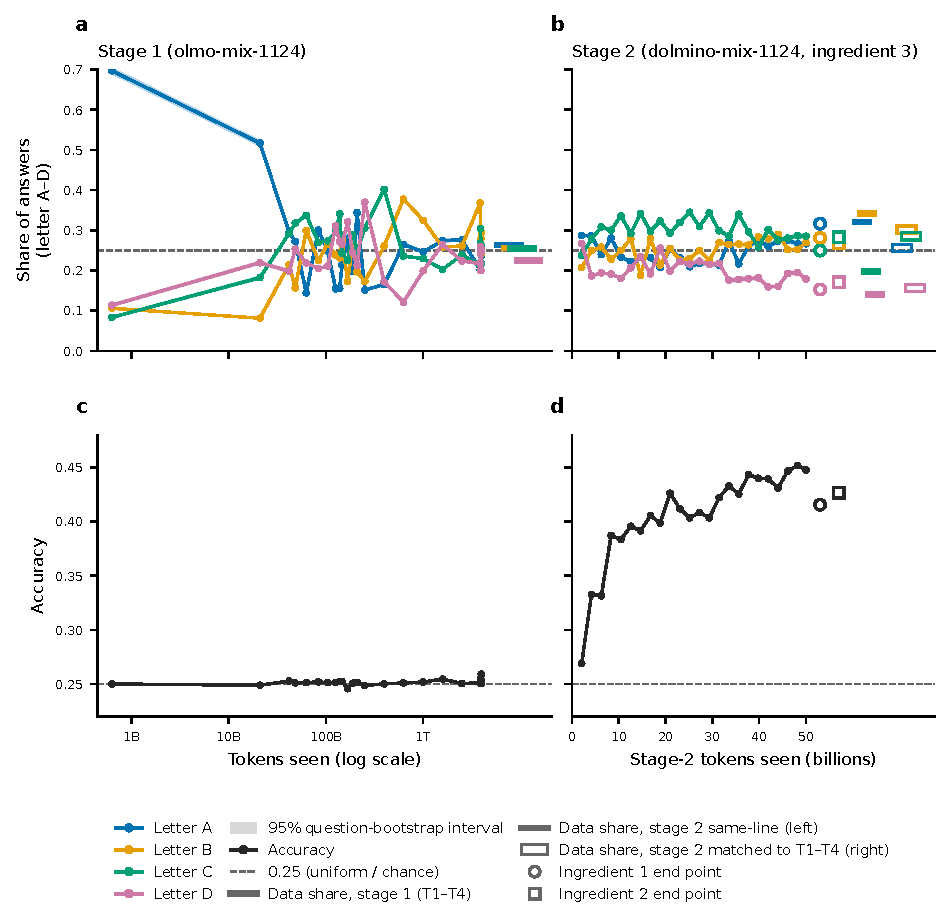
\includegraphics[width=0.92\linewidth]{figures/fig_letter_preference_eos.pdf}
\caption{As Figure~\ref{fig:main}, with an EOS token prepended to every prompt.}\label{fig:eos}
\end{figure}

\section{Audit of the stage-2 count definition}\label{sec:audit}
A random sample of 50 matches of the first definition (strict) was read. In 16 of them a newline separated the cue from the label. Nine of these were \texttt{Answer:}, a newline and \texttt{(A).} followed directly by answer text: the turn marker of a Flan template that alternates \texttt{(Q).} and \texttt{(A).}, not an option label. The 34 same-line matches read as option labels. A full rescan with the forms separated found \MarkerCount{} turn-marker matches, all counted as~A, out of \StrictTotal{} strict matches. The rescan reproduced the first scan's counts exactly. The same-line definition, which excludes these matches, became primary; the strict definition is still reported. The change was made before any test statistic was computed (Appendix~\ref{app:pl}).

\section{Discussion}
The results support four statements:
\begin{itemize}
\item Under the pre-declared test, the change in OLMo~2 1B's letter preference at the stage-1 to stage-2 switch did not match the change in training-data letter shares, under all four data definitions.
\item In this zero-shot letter format, the stage-1 checkpoints answer at chance and are insensitive to option content. Content sensitivity appears only in stage~2.
\item The stage-1 letter preference is not stable: it changes by several points between checkpoints 10{,}000 steps apart.
\item Letter D has the lowest share at all three stage-2 end points under both prefixes, and the lowest share in the stage-2 data under every definition.
\end{itemize}
They do not support the following:
\begin{itemize}
\item That the preference follows the data. With averaged baselines the primary definition ranks first, but two other definitions and the EOS-prefixed series do not, and single-baseline ranks span almost the full range.
\item That the preference does not follow the data. Four labels allow a minimum permutation $p$-value of only $1/24$, and checkpoint-to-checkpoint variation is as large as the shift.
\item That data causes any change at the switch. The learning-rate schedule changes at the same point as the data.
\item Anything about the released \texttt{main} weights from the checkpoint trajectory.
\end{itemize}

\section{Limitations}
\begin{itemize}
\item Stage-2 counts come from the public pool, not the exact 50B-token sample. The web, peS2o and StackExchange counts come from seeded shard samples.
\item Data shares pool answer keys of questions with any number of options, many with two or three, whereas the prompts have four.
\item One benchmark (\NQuestions{} ARC-Challenge test questions), one prompt format, zero-shot.
\item Prompt formatting matters: an EOS prefix moves shares by up to about \EosEffectMax\pp.
\item Bootstrap intervals resample questions only. Checkpoint-level standard errors assume independent checkpoints.
\item The test was revised after it was locked (Appendix~\ref{app:pl}). Every revision is dated and states what was known when it was made.
\end{itemize}

\section{Reproducibility}
The repository contains the prompt builder and prompts, the checkpoint manifest, the inference and checkpoint-health scripts with the Slurm wrappers used, the stage-1 query and stage-2 scan scripts, the assembled per-question tables, the analysis script that produces every result table, and \texttt{report/make\_tables.py}, which generates every number and table in this report from those tables. Inference used one NVIDIA A30 per task: \GpuSweep{} GPU-hours for the main sweep and \GpuTail{} for the additional stage-1 checkpoints.

\bibliographystyle{plainnat}
\bibliography{references}

\appendix
\section{Changes after the test was locked}\label{app:pl}
\begin{longtable}{p{0.06\linewidth}p{0.55\linewidth}p{0.31\linewidth}}
\toprule
Id & Change & Known when it was made \\
\midrule
\endhead
PL1 & EOS-prefixed scoring extended to every checkpoint as a secondary series. & Four-checkpoint gate run. \\
PL2 & Loading record and language-modelling loss recorded for every checkpoint. & Gate run (stage-1 accuracy at chance). \\
PL3 & \texttt{main} reported as a separate point, outside the trajectory. & Gate run. \\
PL4 & Seeded sample of the other stage-2 subsets scanned. & Gate run. \\
PL5 & Ingredients 1 and 2 not swept in full; their end points scored as replicates. & Weight comparison of \texttt{main}. \\
PL6 & Primary stage-2 definition changed from strict to same-line; strict kept alongside. & Flan and math counts under the strict definition; gate run. No test statistic. \\
PL7 & Mix-weighted stage-2 share added as secondary. & As PL6. \\
PL8 & Definition matched to the stage-1 strings added; the headline requires all four definitions to agree. & Stage-1 shares. No rescan count, sweep result or test statistic. \\
PL9 & Six end-of-stage-1 checkpoints added; the headline also requires the seven-checkpoint-mean version to agree. & Full sweep tabulated. No test statistic. \\
\bottomrule
\end{longtable}

\section{Count definitions}\label{app:defs}
Patterns use Python \texttt{re} with \texttt{MULTILINE}; \texttt{X} stands for a label (A--D or 1--4).
{\footnotesize
\begin{verbatim}
Same-line  \b(?:[Aa]nswer|correct (?:option|choice))(?: is)?:?[ \t]?\(?X\)?\.?[ \t]*$
Strict     \b(?:[Aa]nswer|correct (?:option|choice))(?: is)?:?\s?\(?X\)?\.?[ \t]*$
Matched    (?:Answer: X|answer is X\.?|Answer: \(X\))\n
Marker     [Aa]nswer:\n\(X\)\.[ \t]*\n(?=\S)
\end{verbatim}
}
The stage-1 strings are \verb|Answer: X\n|, \verb|answer is X\n|, \verb|answer is X.\n| and \verb|Answer: (X)\n|, tokenised with the index tokenizer (Llama-2). Stage-1 letter counts: A~\CountStageOneA, B~\CountStageOneB, C~\CountStageOneC, D~\CountStageOneD.

\section{Corrections during the study}
\begin{itemize}
\item \emph{Digit labels.} Scoring the first token of each label would have given every digit label the same space token and a share of exactly 0.25. Digits are scored after an appended space token instead.
\item \emph{Precision.} bfloat16 inference was discarded after its disagreement with unbatched inference (0.36 nats).
\item \emph{Stage-2 definition.} See Section~\ref{sec:audit}.
\item \emph{Throttling and downloads.} The infini-gram API throttled concurrent requests; queries were serialised and retried until every one returned an exact count. 254 of 5{,}384 stage-2 shard downloads failed with HTTP~429 on the first pass and succeeded on a second. No shard or checkpoint was skipped.
\end{itemize}

\clearpage
\section{All scored revisions}
\begingroup\scriptsize\setlength{\tabcolsep}{3pt}
\begin{longtable}{lrcccccccccccc}
\caption{Letter shares (shuffled condition) and accuracy at every scored revision. S1 = stage 1, S2-i$k$ = stage 2, ingredient $k$; numbers after the label are training steps. Tokens for \texttt{main} are the manifest value. NLL = mean per-token negative log-likelihood (nats) on the 500 original-order prompts.}\label{tab:allrevs}\\
\toprule
 & & \multicolumn{5}{c}{No prefix} & \multicolumn{5}{c}{EOS prefix} & \\
\cmidrule(lr){3-7}\cmidrule(lr){8-12}
Revision & Tokens (B) & A & B & C & D & Acc. & A & B & C & D & Acc. & NLL \\
\midrule
\endfirsthead
\toprule Revision & Tokens (B) & A & B & C & D & Acc. & A & B & C & D & Acc. & NLL \\ \midrule
\endhead
\bottomrule
\endlastfoot
S1 300 & 0.6 & 0.664 & 0.112 & 0.086 & 0.138 & 0.250 & 0.697 & 0.106 & 0.083 & 0.114 & 0.250 & 6.70 \\
S1 10,000 & 21.0 & 0.513 & 0.072 & 0.197 & 0.217 & 0.249 & 0.517 & 0.081 & 0.182 & 0.219 & 0.249 & 2.42 \\
S1 20,000 & 41.9 & 0.283 & 0.218 & 0.279 & 0.221 & 0.251 & 0.295 & 0.215 & 0.292 & 0.198 & 0.253 & 2.33 \\
S1 23,100 & 48.4 & 0.281 & 0.176 & 0.289 & 0.255 & 0.252 & 0.272 & 0.157 & 0.318 & 0.253 & 0.251 & 2.25 \\
S1 30,000 & 62.9 & 0.158 & 0.275 & 0.296 & 0.271 & 0.248 & 0.144 & 0.300 & 0.337 & 0.219 & 0.251 & 2.22 \\
S1 40,000 & 83.9 & 0.291 & 0.216 & 0.272 & 0.221 & 0.249 & 0.300 & 0.225 & 0.270 & 0.205 & 0.252 & 2.21 \\
S1 50,000 & 104.9 & 0.266 & 0.249 & 0.273 & 0.212 & 0.252 & 0.248 & 0.267 & 0.274 & 0.211 & 0.251 & 2.18 \\
S1 60,000 & 125.8 & 0.148 & 0.243 & 0.312 & 0.298 & 0.250 & 0.155 & 0.239 & 0.296 & 0.311 & 0.251 & 2.23 \\
S1 66,200 & 138.8 & 0.152 & 0.222 & 0.351 & 0.275 & 0.251 & 0.156 & 0.231 & 0.341 & 0.272 & 0.252 & 2.18 \\
S1 70,000 & 146.8 & 0.200 & 0.310 & 0.238 & 0.251 & 0.251 & 0.213 & 0.277 & 0.244 & 0.266 & 0.252 & 2.20 \\
S1 80,000 & 167.8 & 0.286 & 0.175 & 0.230 & 0.309 & 0.252 & 0.280 & 0.173 & 0.225 & 0.321 & 0.246 & 2.17 \\
S1 90,000 & 188.7 & 0.215 & 0.253 & 0.309 & 0.223 & 0.250 & 0.198 & 0.268 & 0.290 & 0.244 & 0.251 & 2.15 \\
S1 100,000 & 209.7 & 0.332 & 0.201 & 0.267 & 0.200 & 0.251 & 0.344 & 0.197 & 0.247 & 0.212 & 0.251 & 2.15 \\
S1 120,000 & 251.7 & 0.155 & 0.181 & 0.332 & 0.332 & 0.246 & 0.152 & 0.173 & 0.306 & 0.370 & 0.249 & 2.15 \\
S1 190,000 & 398.5 & 0.153 & 0.257 & 0.407 & 0.182 & 0.250 & 0.165 & 0.261 & 0.402 & 0.172 & 0.250 & 2.13 \\
S1 300,000 & 629.1 & 0.240 & 0.384 & 0.241 & 0.135 & 0.250 & 0.265 & 0.378 & 0.236 & 0.121 & 0.251 & 2.11 \\
S1 480,000 & 1006.6 & 0.243 & 0.356 & 0.216 & 0.186 & 0.252 & 0.246 & 0.325 & 0.230 & 0.199 & 0.252 & 2.05 \\
S1 760,000 & 1593.8 & 0.287 & 0.263 & 0.228 & 0.222 & 0.251 & 0.275 & 0.258 & 0.203 & 0.265 & 0.255 & 2.09 \\
S1 1,200,000 & 2516.6 & 0.303 & 0.248 & 0.236 & 0.213 & 0.251 & 0.276 & 0.261 & 0.239 & 0.223 & 0.251 & 2.05 \\
S1 1,850,000 & 3879.7 & 0.238 & 0.322 & 0.222 & 0.219 & 0.252 & 0.201 & 0.368 & 0.213 & 0.218 & 0.251 & 2.01 \\
S1 1,860,000 & 3900.7 & 0.218 & 0.263 & 0.272 & 0.247 & 0.251 & 0.209 & 0.263 & 0.268 & 0.260 & 0.255 & 2.02 \\
S1 1,870,000 & 3921.7 & 0.220 & 0.256 & 0.287 & 0.237 & 0.255 & 0.201 & 0.252 & 0.304 & 0.242 & 0.255 & 2.00 \\
S1 1,880,000 & 3942.6 & 0.290 & 0.276 & 0.247 & 0.188 & 0.254 & 0.259 & 0.279 & 0.262 & 0.200 & 0.254 & 1.99 \\
S1 1,890,000 & 3963.6 & 0.290 & 0.227 & 0.229 & 0.254 & 0.252 & 0.248 & 0.242 & 0.258 & 0.252 & 0.253 & 2.01 \\
S1 1,900,000 & 3984.6 & 0.293 & 0.240 & 0.238 & 0.229 & 0.258 & 0.238 & 0.252 & 0.263 & 0.247 & 0.259 & 1.99 \\
S1 1,907,359 & 4000.0 & 0.270 & 0.266 & 0.204 & 0.259 & 0.255 & 0.242 & 0.294 & 0.217 & 0.247 & 0.251 & 2.02 \\
S2-i3 1,000 & 4002.1 & 0.272 & 0.205 & 0.238 & 0.285 & 0.266 & 0.287 & 0.208 & 0.238 & 0.267 & 0.269 & 2.10 \\
S2-i3 2,000 & 4004.2 & 0.258 & 0.267 & 0.266 & 0.208 & 0.333 & 0.286 & 0.249 & 0.278 & 0.187 & 0.333 & 2.12 \\
S2-i3 3,000 & 4006.3 & 0.233 & 0.261 & 0.285 & 0.221 & 0.344 & 0.240 & 0.258 & 0.308 & 0.194 & 0.332 & 2.07 \\
S2-i3 4,000 & 4008.4 & 0.270 & 0.253 & 0.271 & 0.206 & 0.414 & 0.280 & 0.228 & 0.300 & 0.191 & 0.387 & 2.06 \\
S2-i3 5,000 & 4010.5 & 0.234 & 0.271 & 0.295 & 0.200 & 0.400 & 0.233 & 0.250 & 0.336 & 0.180 & 0.384 & 2.06 \\
S2-i3 6,000 & 4012.6 & 0.213 & 0.298 & 0.280 & 0.209 & 0.401 & 0.222 & 0.279 & 0.292 & 0.207 & 0.396 & 2.10 \\
S2-i3 7,000 & 4014.7 & 0.246 & 0.205 & 0.309 & 0.241 & 0.418 & 0.235 & 0.188 & 0.342 & 0.234 & 0.392 & 2.21 \\
S2-i3 8,000 & 4016.8 & 0.227 & 0.281 & 0.283 & 0.209 & 0.428 & 0.232 & 0.279 & 0.298 & 0.192 & 0.406 & 2.16 \\
S2-i3 9,000 & 4018.9 & 0.203 & 0.222 & 0.312 & 0.263 & 0.415 & 0.208 & 0.214 & 0.323 & 0.256 & 0.399 & 2.13 \\
S2-i3 10,000 & 4021.0 & 0.248 & 0.265 & 0.264 & 0.224 & 0.444 & 0.253 & 0.255 & 0.293 & 0.199 & 0.426 & 2.12 \\
S2-i3 11,000 & 4023.1 & 0.237 & 0.257 & 0.281 & 0.226 & 0.439 & 0.232 & 0.226 & 0.320 & 0.222 & 0.412 & 2.15 \\
S2-i3 12,000 & 4025.2 & 0.254 & 0.250 & 0.281 & 0.215 & 0.448 & 0.209 & 0.230 & 0.345 & 0.216 & 0.404 & 2.11 \\
S2-i3 13,000 & 4027.3 & 0.220 & 0.259 & 0.281 & 0.240 & 0.427 & 0.218 & 0.250 & 0.309 & 0.223 & 0.409 & 2.17 \\
S2-i3 14,000 & 4029.4 & 0.243 & 0.264 & 0.284 & 0.210 & 0.437 & 0.217 & 0.225 & 0.343 & 0.215 & 0.404 & 2.16 \\
S2-i3 15,000 & 4031.5 & 0.234 & 0.300 & 0.248 & 0.218 & 0.439 & 0.214 & 0.269 & 0.299 & 0.218 & 0.422 & 2.12 \\
S2-i3 16,000 & 4033.6 & 0.285 & 0.264 & 0.241 & 0.211 & 0.433 & 0.274 & 0.265 & 0.286 & 0.176 & 0.433 & 2.12 \\
S2-i3 17,000 & 4035.7 & 0.246 & 0.303 & 0.259 & 0.193 & 0.441 & 0.217 & 0.266 & 0.340 & 0.178 & 0.425 & 2.12 \\
S2-i3 18,000 & 4037.8 & 0.266 & 0.269 & 0.254 & 0.211 & 0.453 & 0.261 & 0.264 & 0.296 & 0.180 & 0.444 & 2.12 \\
S2-i3 19,000 & 4039.9 & 0.274 & 0.304 & 0.222 & 0.199 & 0.438 & 0.276 & 0.284 & 0.258 & 0.182 & 0.440 & 2.13 \\
S2-i3 20,000 & 4042.0 & 0.267 & 0.297 & 0.248 & 0.188 & 0.445 & 0.260 & 0.279 & 0.301 & 0.159 & 0.440 & 2.12 \\
S2-i3 21,000 & 4044.1 & 0.272 & 0.309 & 0.232 & 0.186 & 0.427 & 0.273 & 0.290 & 0.276 & 0.161 & 0.431 & 2.11 \\
S2-i3 22,000 & 4046.2 & 0.273 & 0.272 & 0.239 & 0.216 & 0.452 & 0.275 & 0.252 & 0.281 & 0.192 & 0.447 & 2.13 \\
S2-i3 23,000 & 4048.3 & 0.265 & 0.273 & 0.247 & 0.216 & 0.456 & 0.266 & 0.253 & 0.287 & 0.195 & 0.452 & 2.12 \\
S2-i3 23,852 & 4050.0 & 0.262 & 0.288 & 0.244 & 0.205 & 0.451 & 0.266 & 0.270 & 0.285 & 0.179 & 0.448 & 2.12 \\
S2-i1 23,852 & 4050.0 & 0.273 & 0.305 & 0.240 & 0.182 & 0.437 & 0.317 & 0.281 & 0.250 & 0.153 & 0.416 & 2.17 \\
S2-i2 23,852 & 4050.0 & 0.263 & 0.300 & 0.256 & 0.181 & 0.425 & 0.279 & 0.267 & 0.283 & 0.171 & 0.427 & 2.18 \\
main & 4050.0 & 0.185 & 0.238 & 0.362 & 0.215 & 0.374 & 0.232 & 0.241 & 0.322 & 0.206 & 0.403 & 2.08 \\
\end{longtable}

\endgroup

\end{document}
